\begin{figure}[H]
\centering
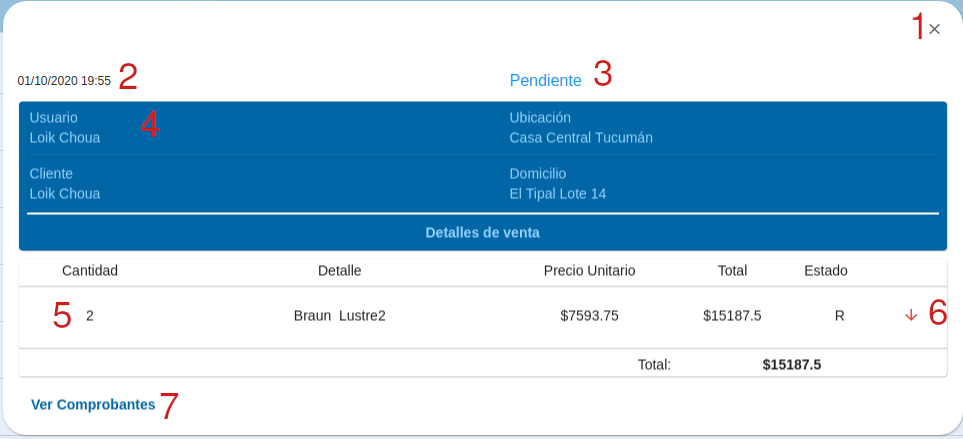
\includegraphics[width=\textwidth,height=\textheight,keepaspectratio]{Escenarios/AD-12-00}
\caption{Escenario - AD-12-00}
\label{fig:AD-12-00}
\end{figure}
Este es el escenario que muestra información más detallada de una venta a los usuarios.
Con el botón \textbf{AD-12-01} se podrá cerrar la ventana y volver al escenario \textbf{AD-10-00}. El campo \textbf{AD-12-02} muestra la fecha en la que fue creada la venta y el campo \textbf{AD-12-03} muestra el estado en el cual se encuentra la venta.
La sección \textbf{AD-12-04} muestra información relacionada al cliente, al empleado que creo la venta, la ubicación en la cual fue creado y cual es la dirección de entrega especificada para el cliente.
En la sección \textbf{AD-12-05} se muestra infomación de las líneas de venta, como la cantidad, el detalle, el precio unitario, el total y el estado de la linea de venta. Un click en el boton \textbf{AD-12-06} permite cancelar una linea de venta. Un click en el boton \textbf{AD-12-07} navegará al escenario \textbf{AD-14-00} para ver los comprobantes de la venta. 
\\